\documentclass[aspectratio=169,11pt]{beamer}
\usetheme{Madrid}
\usecolortheme{default}
\definecolor{MainBlue}{RGB}{30,65,110}
\setbeamercolor{structure}{fg=MainBlue}
\setbeamercolor{title}{bg=MainBlue,fg=white}
\setbeamercolor{frametitle}{bg=MainBlue,fg=white}
\setbeamertemplate{navigation symbols}{}
\setbeamertemplate{footline}[frame number]
\setbeamertemplate{items}[circle]
\usepackage[T1]{fontenc}
\usepackage{lmodern,amsmath,amssymb,bm,graphicx,booktabs}
\graphicspath{{Plots/}}
\title[STAT 204 Project]{Predicting appliance energy use}
\subtitle{STAT 204 Project\\[0.5em]\small A reproduction and extension of Candanedo, Feldheim, and Deramaix (2017)}
\author{Hangyu Li}
\institute{Department of Statistics\\University of California, Santa Cruz}
\date{November 3, 2026}
\begin{document}
\begin{frame}
\titlepage
\end{frame}

\begin{frame}{Background and research questions}
Household appliances account for approximately 30\% of residential electricity consumption in the United States.\footnote{\scriptsize Cetin et al.\ (2014). Full reference on the final slide.} Predicting when households use that electricity can inform demand planning.
\medskip
\begin{enumerate}
\item Can we reproduce the paper's ordinary least squares (OLS) results for a low-energy house?
\item Can we improve prediction by combining correlated sensor readings through principal component regression (PCR)?
\item When predicting a later interval, how much does the most recent appliance reading help?
\end{enumerate}
\end{frame}

\begin{frame}{Data overview}
\textbf{19,735 consecutive 10-minute intervals} from one house, January--May 2016 (137 days). The response is appliance energy use in each interval, measured in watt-hours (Wh).
\medskip

\begin{tabular}{@{}lp{.70\linewidth}@{}}
\toprule
Source & Predictors\\\midrule
Lighting & Lighting energy use in the same interval (Wh)\\[.4em]
Household sensors & Temperature and relative humidity at nine locations, including one outside the house\\[.4em]
Airport weather & Temperature, humidity, pressure, wind speed, visibility, and dew point, interpolated to 10-minute intervals\\[.4em]
Calendar & Seconds since midnight, day of the week, and weekday/weekend status\\
\bottomrule
\end{tabular}
\end{frame}

\begin{frame}{Reproduction of the published OLS model}
We matched the authors' 75/25 random split, stratified by appliance use, and used 10-fold cross-validation repeated three times within the training set.
\medskip
\begin{center}
\begin{tabular}{@{}lrr@{}}
\toprule
Held-out test metric & Published & Reproduced\\\midrule
RMSE (Wh) & 93.18 & 93.18\\
MAE (Wh) & 51.97 & 51.97\\
$R^2$ & 0.16 & 0.159\\
MAPE (\%) & 59.93 & 59.94\\
\bottomrule
\end{tabular}
\end{center}
The model explains about 16\% of test-set variation. Across 30 random splits, test RMSE averaged 93.5 Wh (SD 2.5 Wh).
\end{frame}

\begin{frame}{OLS underpredicts high-use intervals}
\begin{columns}[c,onlytextwidth]
\column{.58\textwidth}
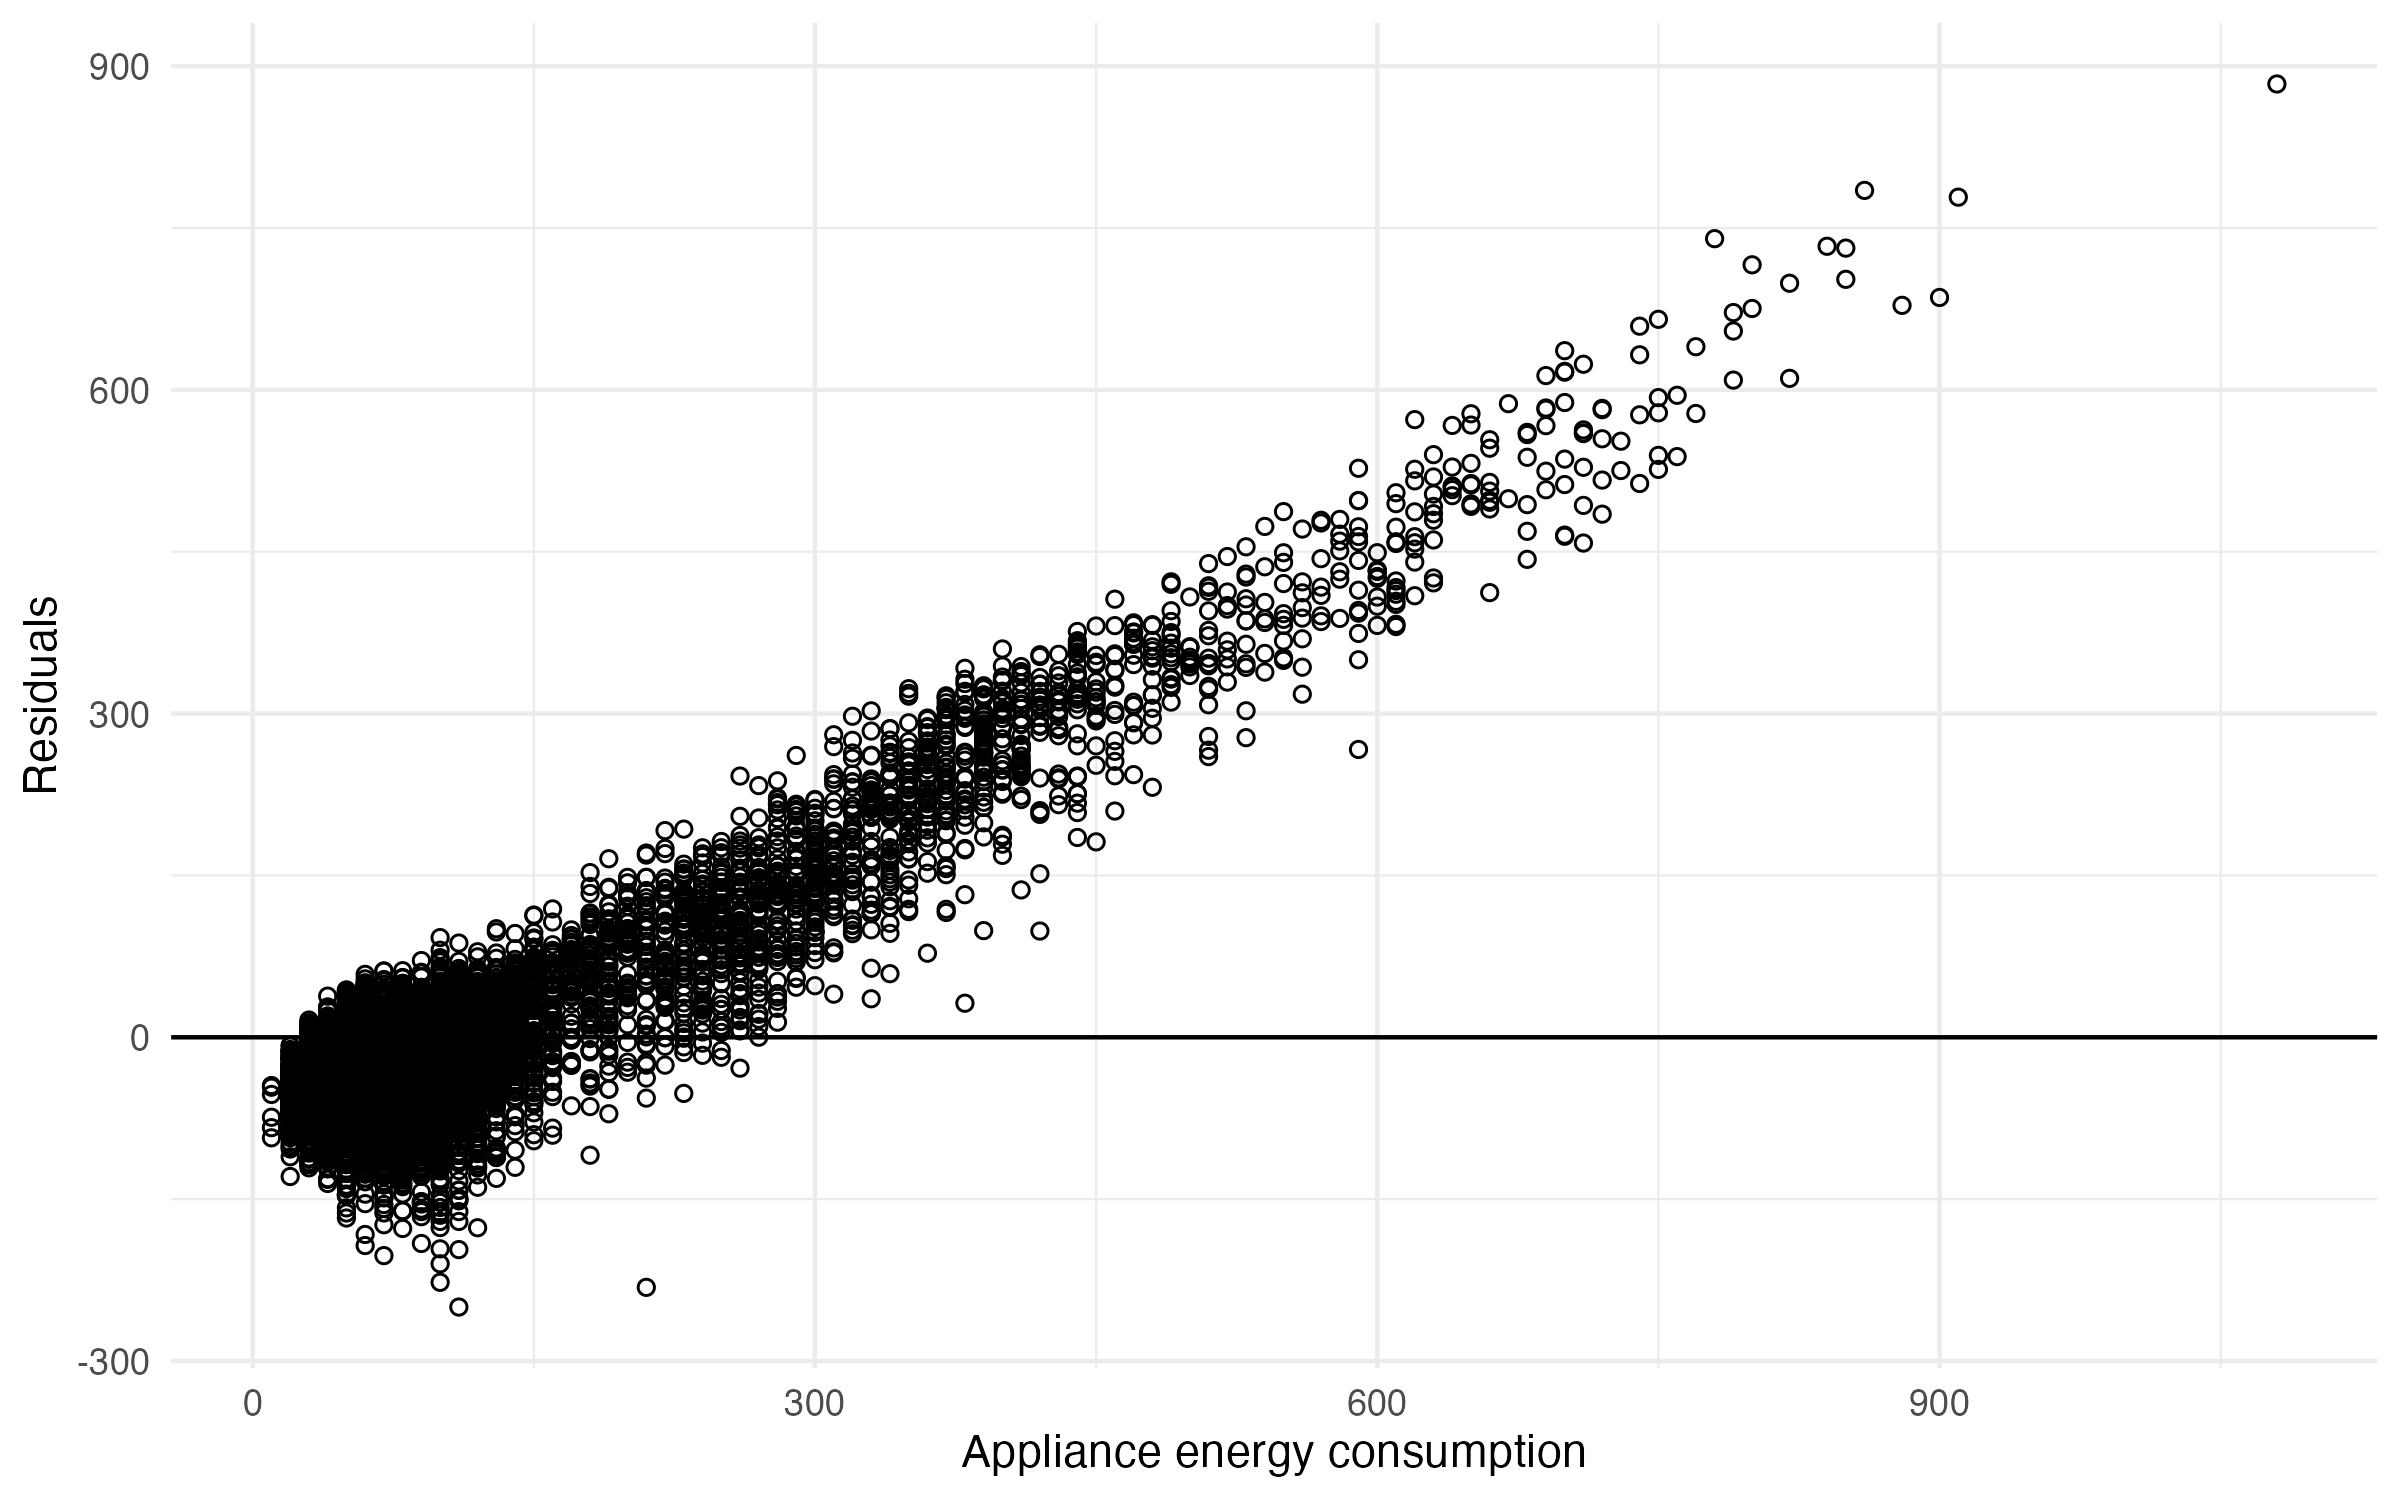
\includegraphics[width=\linewidth]{02-residuals-observed.png}
\column{.39\textwidth}
Each point is a training interval. Its residual is observed minus fitted energy use.
\medskip

At the highest observed loads, the residuals are large and positive. OLS substantially underestimates those peaks.
\medskip

Large misses receive extra weight in RMSE, helping explain the gap between test RMSE (93 Wh) and MAE (52 Wh).
\end{columns}
\end{frame}

\begin{frame}{Multicollinearity Among Predictors}
    \begin{columns}[c,onlytextwidth]
        \column{0.59\textwidth}
            \centering\small
            \textbf{Correlations across indoor locations}\par\smallskip
            \begin{tabular}{@{}lrrr@{}}
                \toprule
                Sensor pairs & Min & Median & Max \\
                \midrule
                Temperature & 0.58 & 0.85 & 0.94 \\
                Relative humidity & 0.25 & 0.78 & 0.90 \\
                \bottomrule
            \end{tabular}\par\medskip
            \textbf{Five largest indoor VIFs in full OLS}\par\smallskip
            \begin{tabular}{@{}lr@{}}
                \toprule
                Predictor & VIF \\
                \midrule
                T9 & 29.49 \\
                T2 & 29.00 \\
                RH\_2 & 21.89 \\
                T1 & 20.20 \\
                RH\_4 & 17.81 \\
                \bottomrule
            \end{tabular}\par\smallskip
            {\scriptsize VIFs above 10 commonly flag strong collinearity.\par}
        \column{0.38\textwidth}
            \small
            Across the 28 pairs of indoor locations, temperatures tend
            to rise and fall together. Relative humidity follows a similar
            pattern, with more variation across pairs.

            \medskip
            Can two components summarize temperature and humidity
            across the house?
    \end{columns}
\end{frame}

% ---------- PCA / PCR ----------
\begin{frame}{PCA Setup}
    We fit PCA on standardized training predictors and kept
    \textit{day of the week} as a factor in every regression.

    \medskip
    \begin{columns}[T,onlytextwidth]
        \begin{column}{0.48\textwidth}
            \centering
            \textbf{Full PCR: 26 numeric predictors}\par
            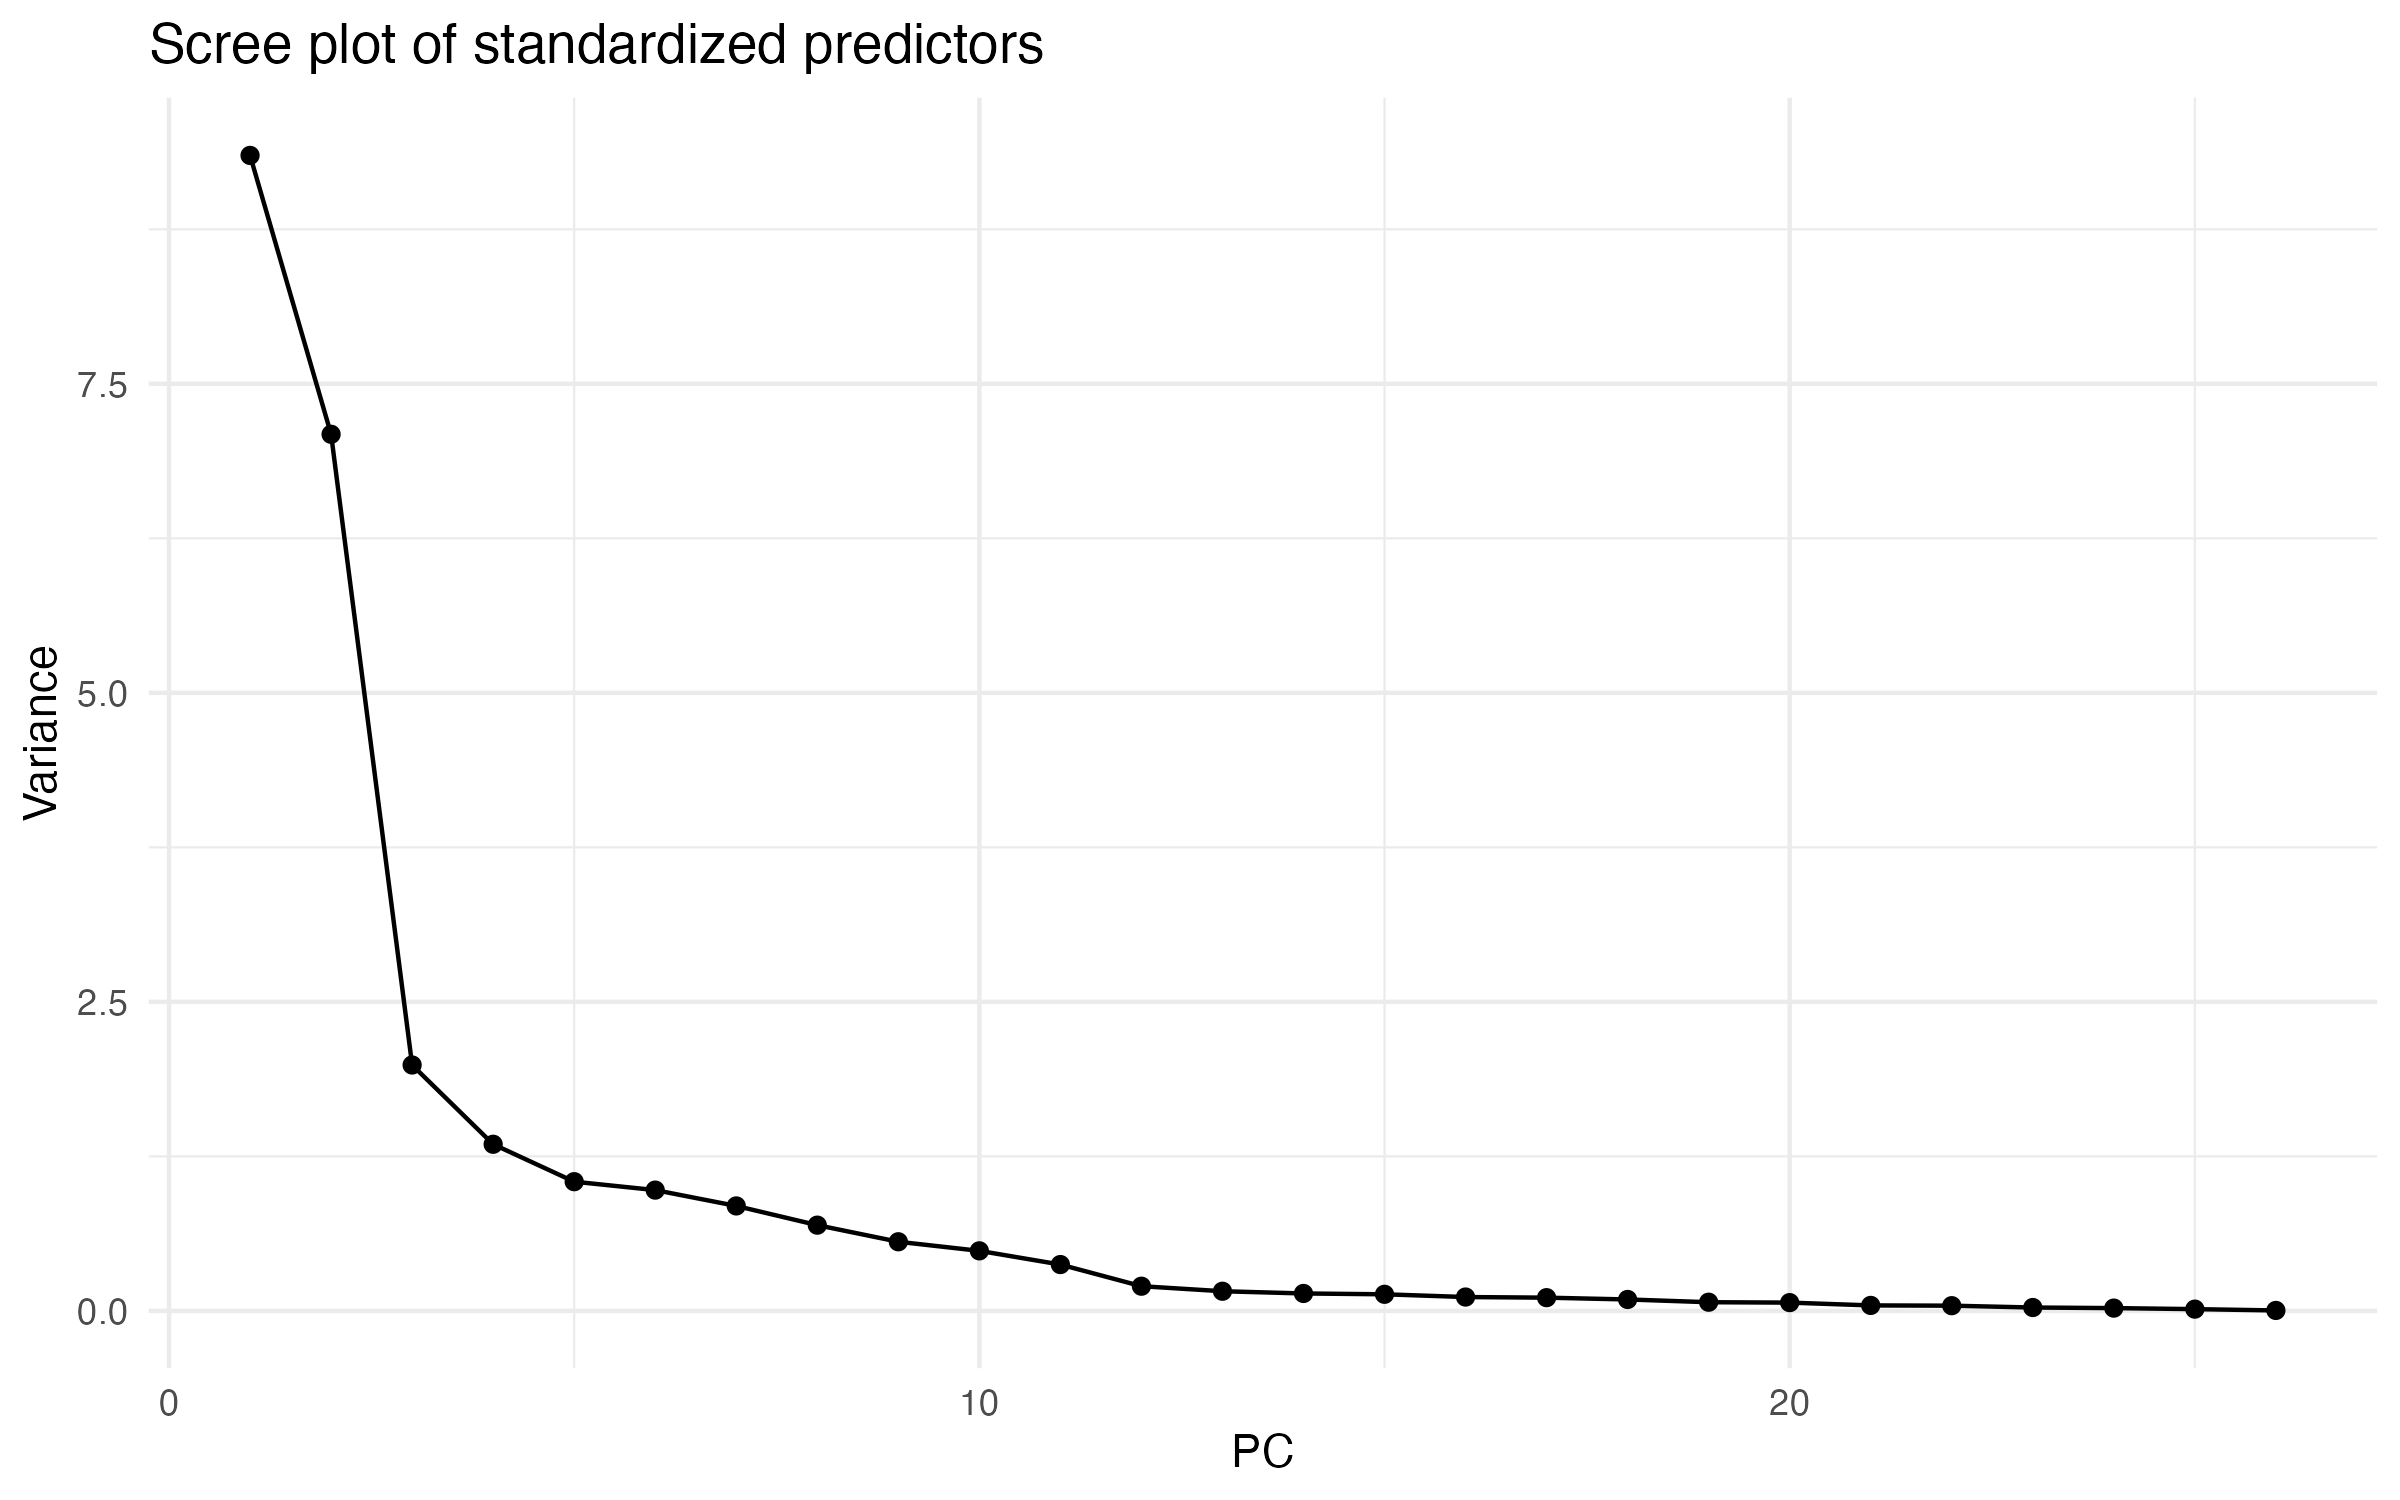
\includegraphics[width=\linewidth,height=0.27\textheight,
                             keepaspectratio]{02-predictor-scree.png}
            \begin{itemize}\small
                \item \textbf{3 PCs.} The scree plot begins to flatten around PC3.
                \item \textbf{5 PCs.} Five is the smallest number that captures at least 80\% of the variance (80.1\%).
            \end{itemize}
        \end{column}
        \begin{column}{0.48\textwidth}
            \centering
            \textbf{Indoor PCR: 16 indoor features}\par
            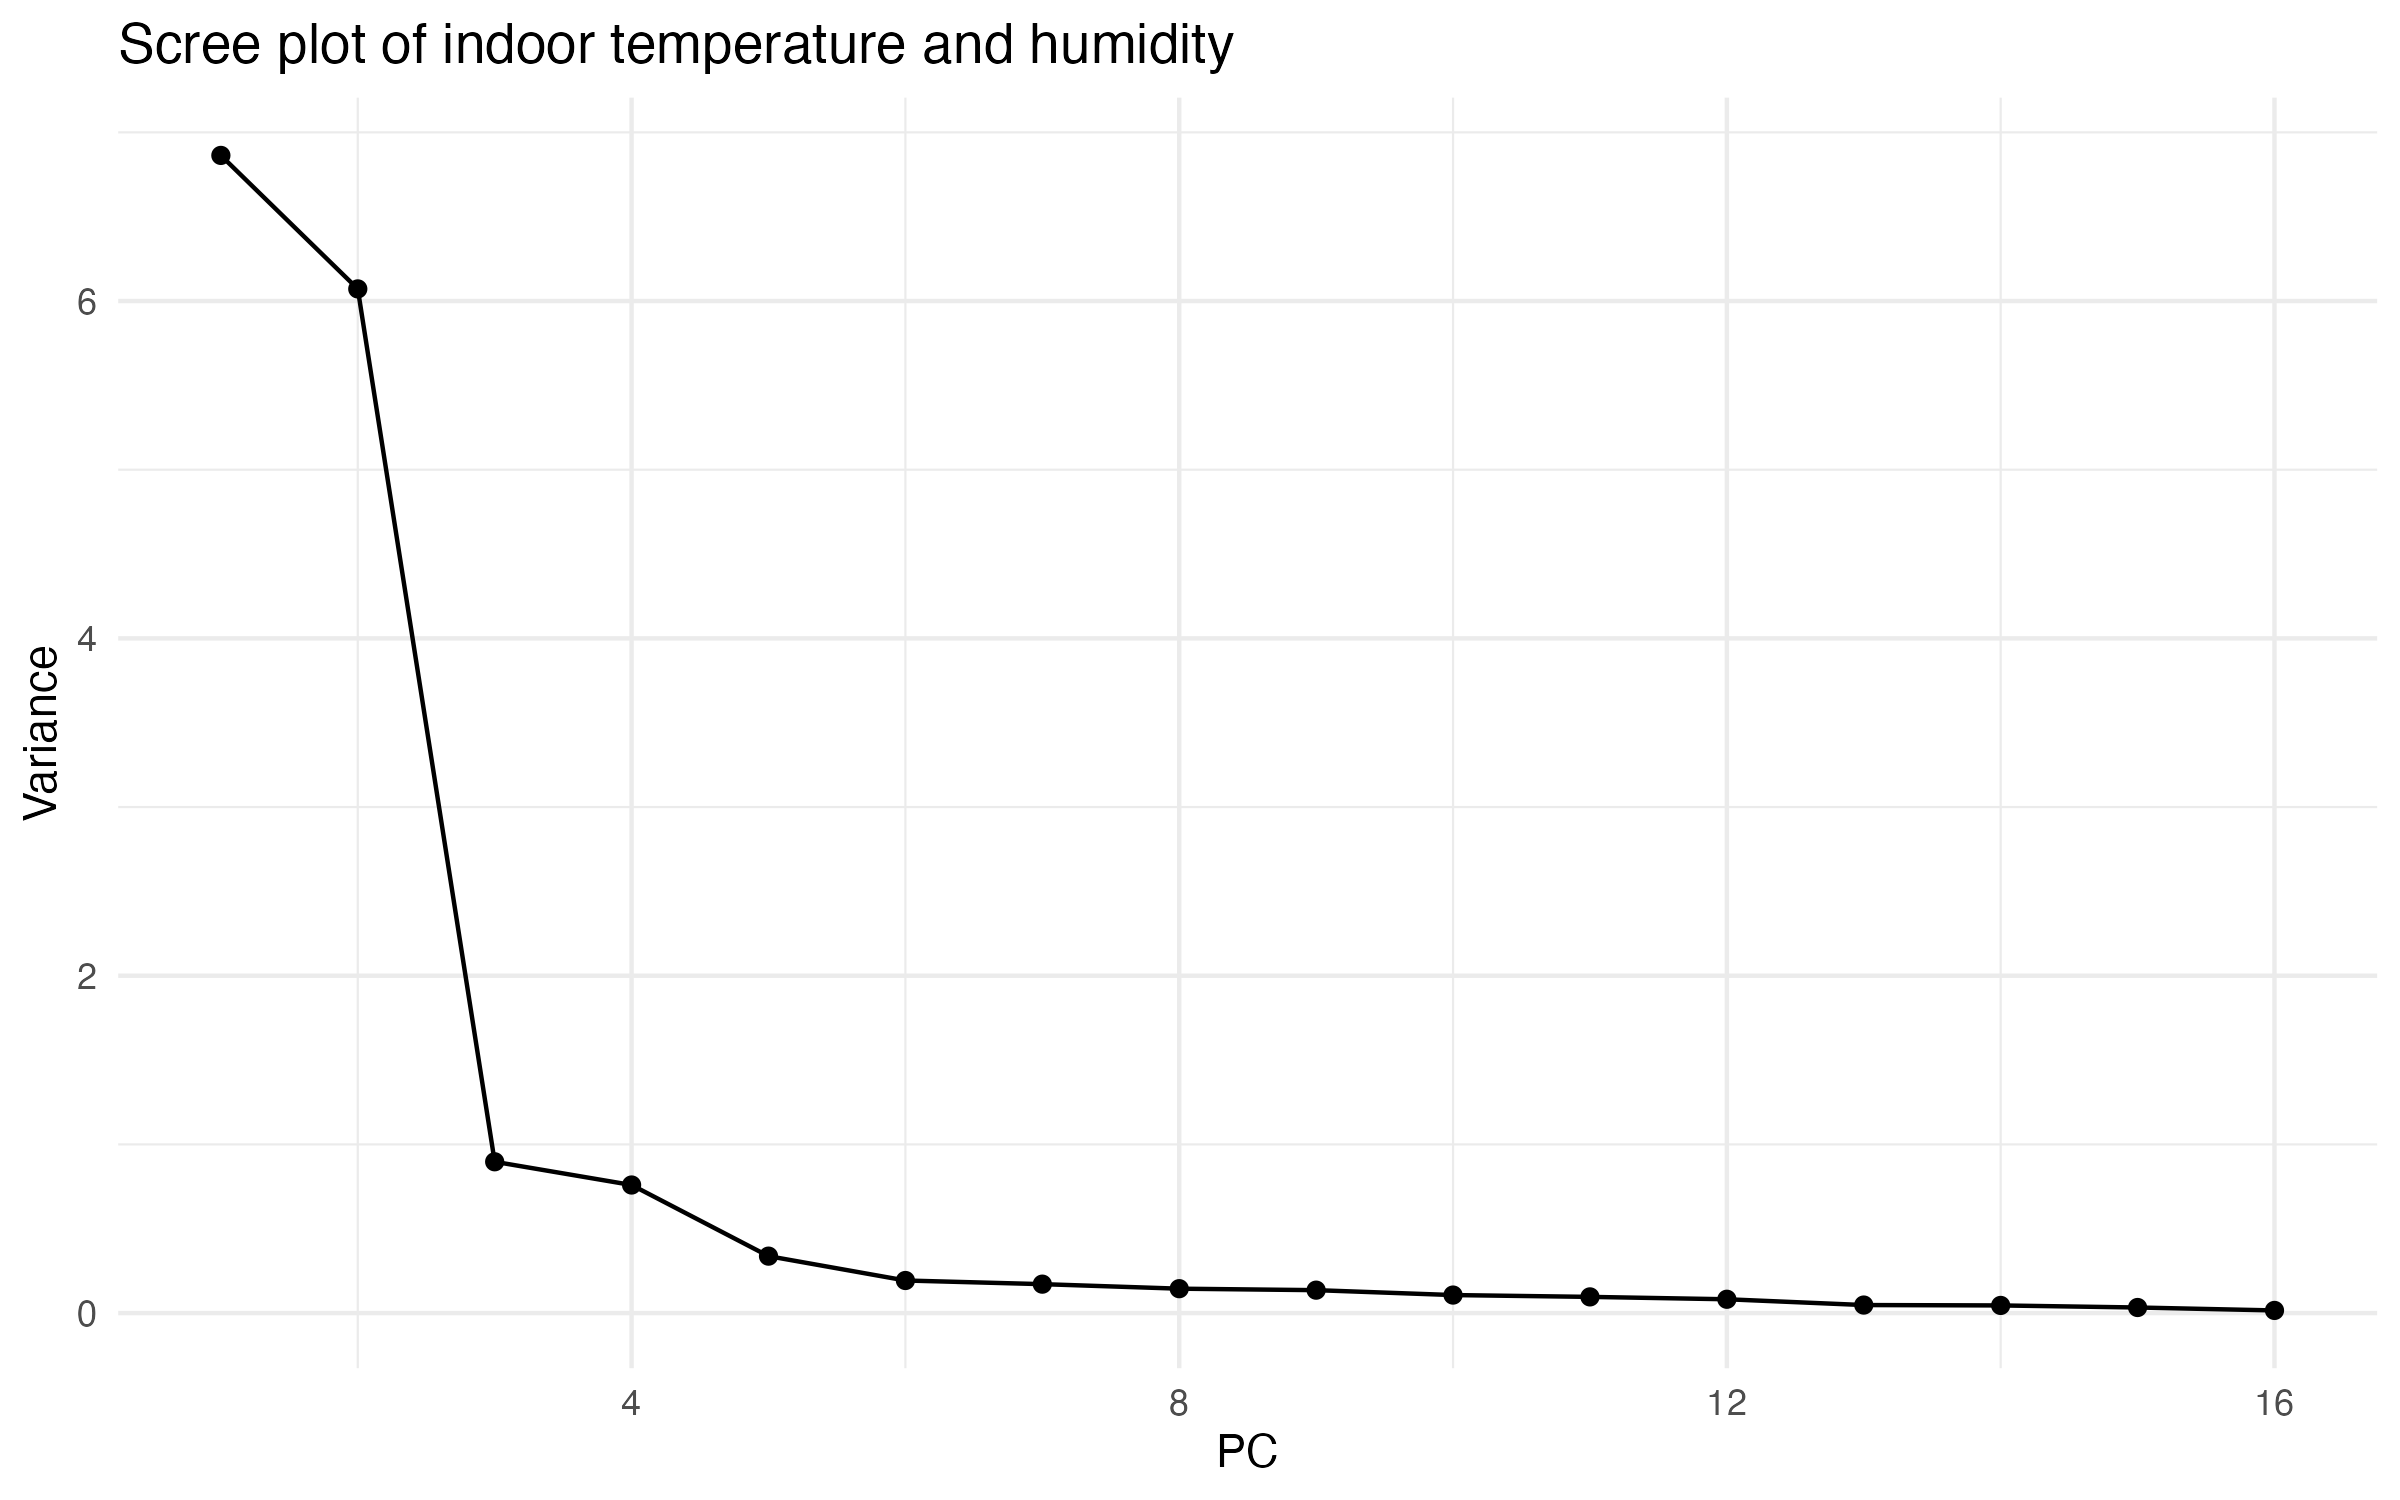
\includegraphics[width=\linewidth,height=0.27\textheight,
                             keepaspectratio]{03-indoor-scree.png}
            \begin{itemize}\small
                \item \textbf{PC1: temperature.} All eight temperature loadings are positive (0.31--0.36).
                \item \textbf{PC2: humidity.} Humidity loadings range from 0.17 to 0.39, with temperature loadings near zero.
            \end{itemize}
        \end{column}
    \end{columns}
    \smallskip
    {\small The two indoor PCs capture 80.8\% of indoor sensor variance.
    All other predictors enter the indoor PCR model directly.}
\end{frame}

\begin{frame}{PCR Results on the Published Test Split}
    We evaluated all four models shown on the same held-out observations.

    \begin{center}
        \renewcommand{\arraystretch}{1.2}
        \begin{tabular}{@{}lrrr@{}}
            \toprule
            Model & RMSE (Wh) & MAE (Wh) & $R^2$ \\
            \midrule
            OLS                      & \textbf{93.2} & \textbf{52.0} & \textbf{0.159} \\
            Full PCR, 3 components   & 98.7 & 56.2 & 0.055 \\
            Full PCR, 5 components   & 97.2 & 54.1 & 0.085 \\
            Indoor PCR, 2 components & 96.1 & 54.0 & 0.106 \\
            \bottomrule
        \end{tabular}
    \end{center}

    \begin{itemize}
        \item \textbf{Full PCR.} Reducing all 26 numeric predictors to
              five components increased test RMSE by 4.0 Wh.
        \item \textbf{Indoor PCR.} Replacing 16 sensor readings with a
              temperature score and a humidity score increased test RMSE
              by 2.9 Wh relative to OLS.
    \end{itemize}
\end{frame}

\begin{frame}{Time-series evaluation on later observations}
\textbf{Prediction setting.} Estimate appliance use $y_t$ with the previous 10-minute reading $y_{t-1}$ and current sensor and lighting measurements $x_t$ available.
\medskip

\begin{tabular}{@{}ll@{}}
\toprule
Model & Prediction at interval $t$\\\midrule
OLS & $\hat\beta_0+x_t^\top\hat\beta$\\
Persistence & $y_{t-1}$\\
OLS + lag 1 & $\hat\alpha_0+x_t^\top\hat\alpha+\hat\phi\,y_{t-1}$\\\bottomrule
\end{tabular}
\medskip

We trained on the earliest 75\% (14,800 usable intervals after forming the lag) and evaluated all three methods on the same final 4,934 intervals, April 23--May 27. Each prediction uses the latest observed appliance reading when needed.
\end{frame}

\begin{frame}{The previous reading improves prediction}
\begin{center}
\begin{tabular}{@{}lrrr@{}}
\toprule
Chronological test split & RMSE (Wh) & MAE (Wh) & $R^2$\\\midrule
OLS & 84.4 & 52.6 & 0.085\\
Persistence & 64.5 & \textbf{25.8} & 0.466\\
OLS + lag 1 & \textbf{60.3} & 28.3 & \textbf{0.534}\\\bottomrule
\end{tabular}
\end{center}
\medskip
\begin{itemize}
\item Persistence beats OLS on both error measures. The previous reading carries information about ongoing appliance use that the current covariates alone miss.
\item Relative to persistence, OLS + lag 1 lowers RMSE by 4.2 Wh but raises MAE by 2.5 Wh. It performs better when large errors receive extra weight.
\end{itemize}
\end{frame}

\begin{frame}{Adding one lag removes much of the residual dependence}
\centering
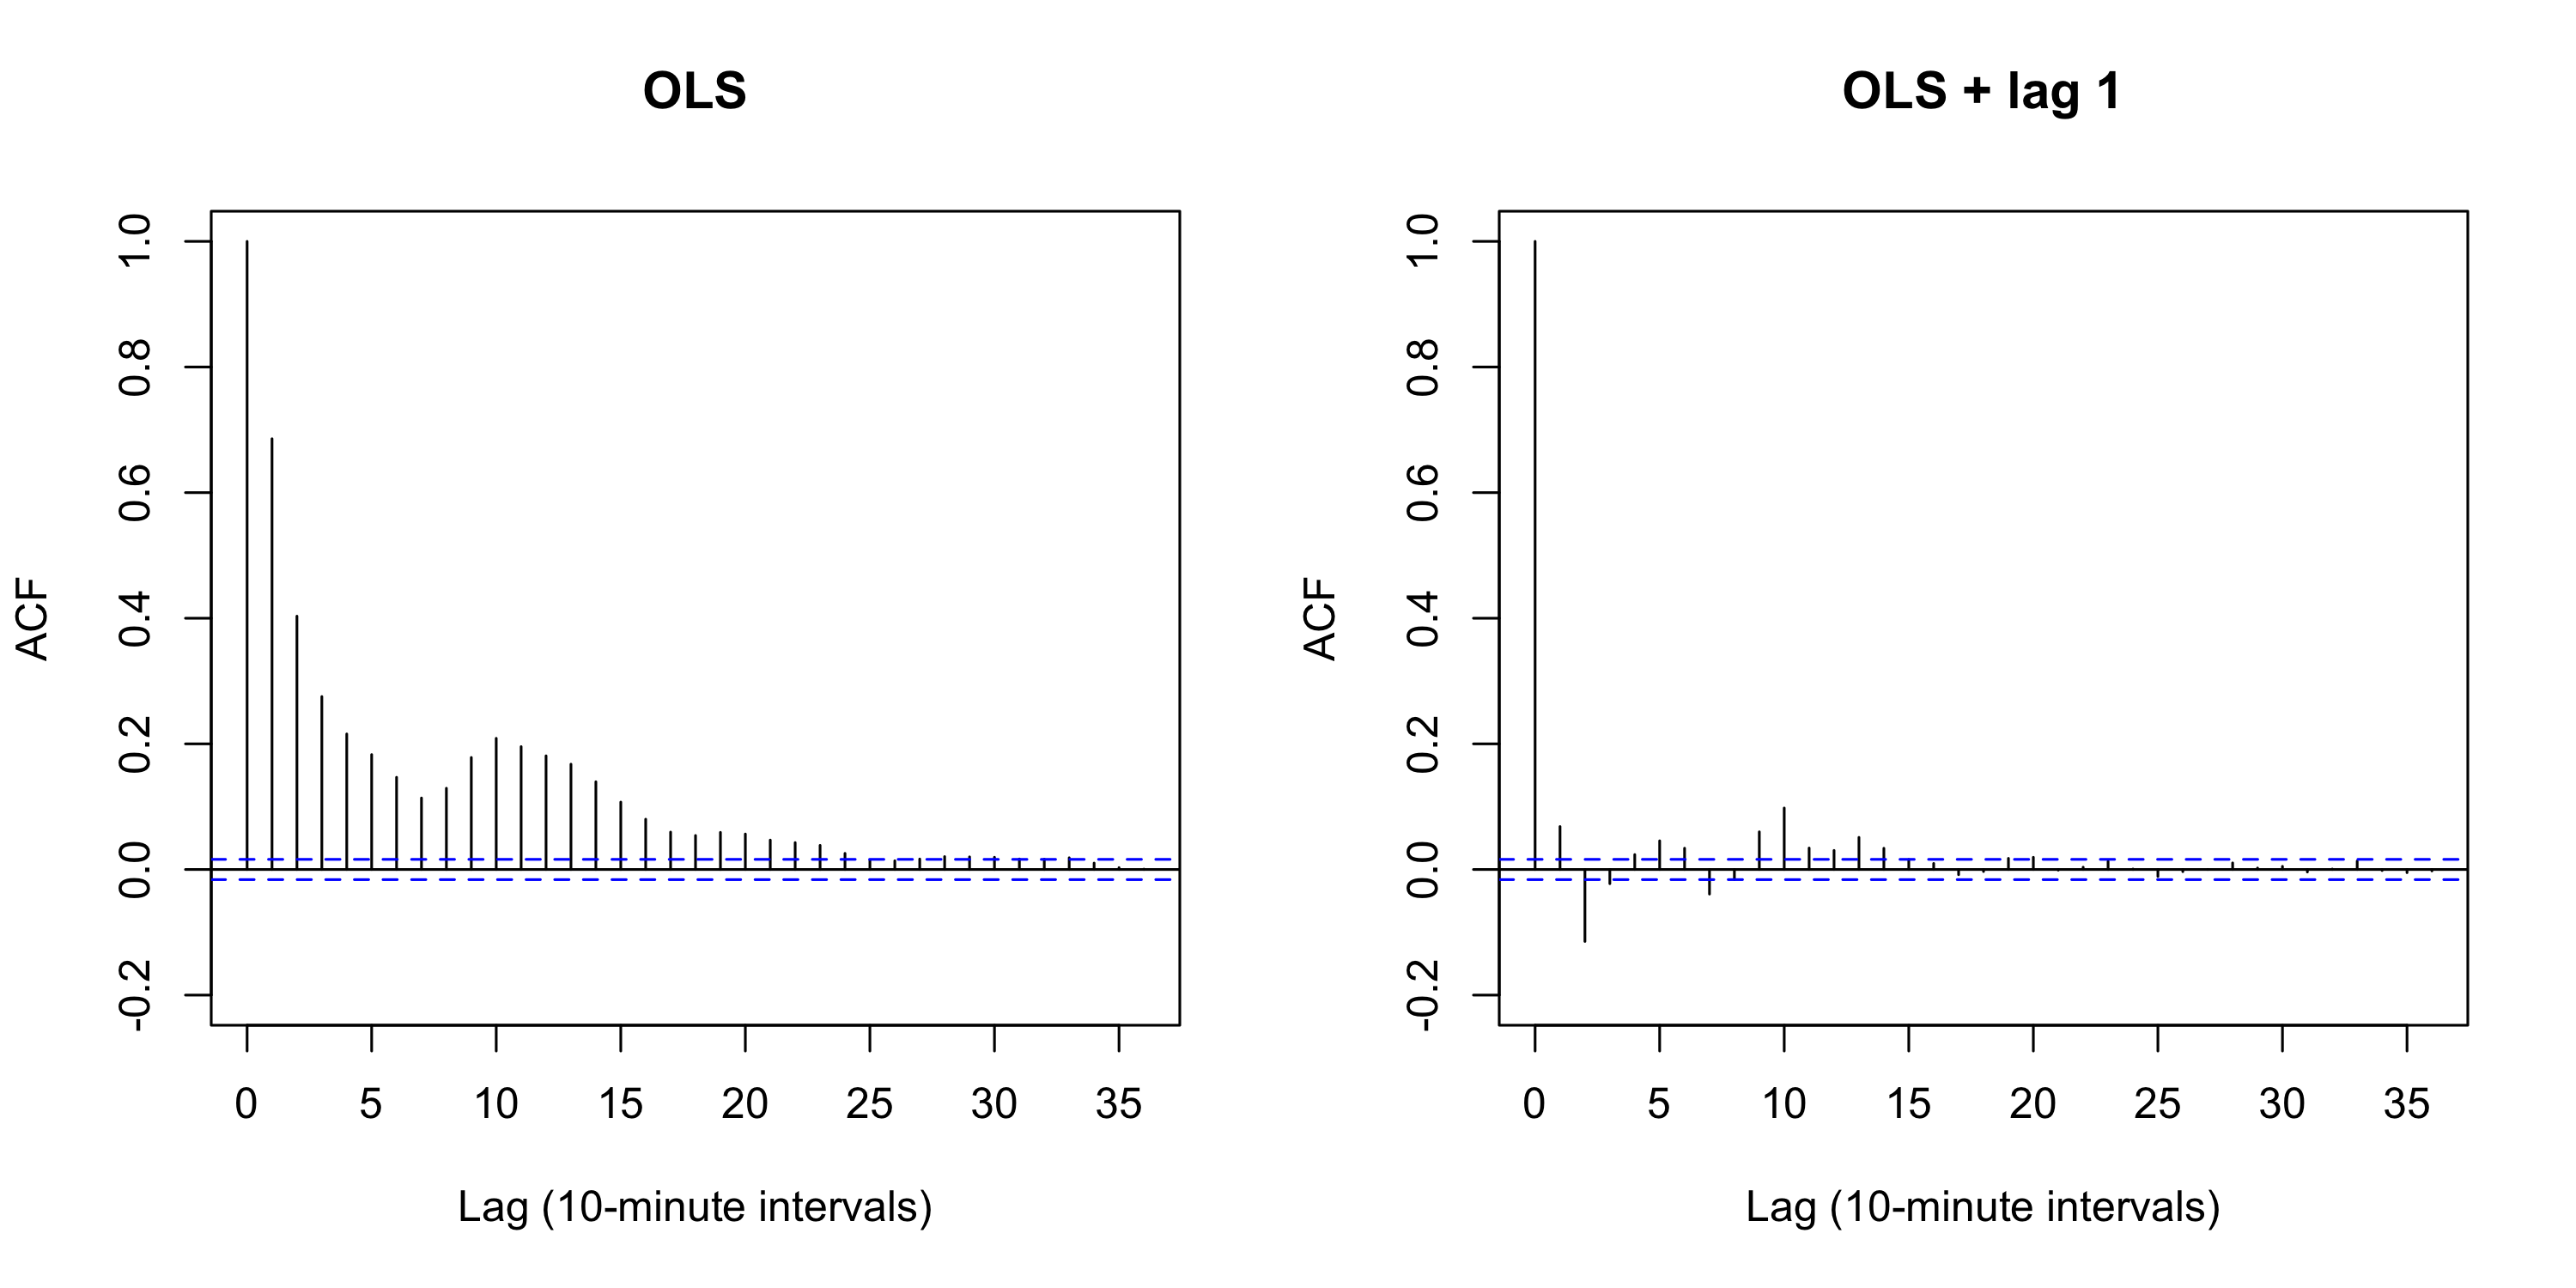
\includegraphics[width=.76\linewidth,height=.56\textheight,keepaspectratio]{04-residual-acf.png}

\medskip
\parbox{.90\linewidth}{On the chronological training set, residual autocorrelation at 10 minutes drops from \textbf{0.686} to \textbf{0.068}. Some dependence remains at later lags.}
\end{frame}

\begin{frame}{Conclusions}
\begin{enumerate}
\item \textbf{Reproduction.} The original OLS results are reproducible, including a test RMSE of 93.18 Wh. The model misses high-use intervals.
\item \textbf{Dimension reduction.} Sensor readings overlap, but each PCR specification increases prediction error on the published random test split.
\item \textbf{Short-term prediction.} On the later test period, the previous appliance reading is especially informative. OLS + lag 1 minimizes RMSE, while persistence minimizes MAE.
\end{enumerate}
\medskip
These results describe one house over 137 days. The lagged regression assumes access to current covariates and an observed appliance reading every ten minutes.
\end{frame}

\begin{frame}{References}
\footnotesize
\begin{thebibliography}{9}
\bibitem{candanedo2017}
Candanedo, L. M., Feldheim, V., and Deramaix, D. (2017).
\newblock Data driven prediction models of energy use of appliances in a low-energy house.
\newblock \emph{Energy and Buildings}, 140, 81--97.
\bibitem{cetin2014}
Cetin, K. S., Tabares-Velasco, P. C., and Novoselac, A. (2014).
\newblock Appliance daily energy use in new residential buildings: Use profiles and variation in time-of-use.
\newblock \emph{Energy and Buildings}, 84, 716--726.
\bibitem{data}
Candanedo, L. M. \href{https://github.com/LuisM78/Appliances-energy-prediction-data}{\textcolor{MainBlue}{Appliances energy prediction data and original R scripts}}.
\end{thebibliography}
\end{frame}
\end{document}
